% Testing and integration
% This chapter should describe the testing and integration of the project.
% What is the testing and integration of the project? What is it intended to achieve?
% How should I go about testing and integrating the project?
% What are the testing requirements of the project?
% What did I actually do?
% What did I need to do differently from my initial plan?
\subsection{Testing}

The testing of the project was conducted in three main stages: unit testing; integration testing; and standalone testing. The unit testing was conducted using .NET Unit testing framework, integration testing was conducted using the Visual Studio IDE, and standalone testing was conducted by running the application in a standalone environment.

\subsubsection{Unit testing}
Unit tests were the primary method of testing the project. Unit tests are particularly useful for an algorithmic system as it allows for the testing of individual components in isolation. In addition to this regression testing, which is the process of testing a program to ensure that changes to one part of the program have not affected other parts of the program, has been used. This testing pattern is particularly useful for this project as it has been build in a modular fashion.

To ensure that the custom regex engine was robust, a comprehensive set of unit tests were written. These tests were designed to test the engine under a variety of conditions, including invalid inputs and a plethora of inputs to be converted to various output formats. The tests that were designed to validate the conversion process used a series of common naming patterns such as camel case, snake case, and pascal case. These tests were as simple as providing the custom engine with an input and comparing the output to an expected result to ensure that the engine was functioning correctly and as expected.

For testing the code analyzers and fix providers the MSBuild testing framework was used. This framework provides the basic functionality to compile input source files, run the analyzers and fix providers on the compiled source files and then compare the generated diagnostics and fixes to expected results provided by the test.
This framework requires a custom format for the test data as described by the documentation on the Microsoft website. The format that the framework desires is not ideal as it produces a lot of duplicated code, so to reduce this a custom source file parser was created to drastically cut down the amount of code that was required to write the tests. In this custom source file parser, the source file can contain code and diagnostic comments. The diagnostic comments are formatted as seen in Table \ref{tab:FileParserSyntax}.
\begin{table}[H]
    \centering
    \caption{File Parser Syntax}
    \label{tab:FileParserSyntax}
    \begin{tabular}{|p{3.5cm}|p{8cm}|p{4cm}|}
        % \hline
        % \multicolumn{3}{|c|}{File Parser Syntax} \\
        \hline
        Syntax&Description&Example\\
        \hline
        \texttt{//\#\textless Diagnostic ID\textgreater}&Indicates the start of a diagnostic block&\texttt{//\#RFSA0001}\\
        \texttt{//-\textless Code\textgreater}&Indicates code that should be removed from the source file&\texttt{//- void Test()}\\
        \texttt{//+\textless Code\textgreater}&Indicates code that should be added to the source file&\texttt{//+ private void Test()}\\
        \texttt{//''\textless Code\textgreater''}&Indicates the area that the diagnostic should occur&\texttt{//- return 2''+''3; }\\
        \hline
    \end{tabular}
\end{table}

The file interpreter creates three copies of the source file in memory for the analyzer input, code fix input and expected output. The source file is then parsed for diagnostic comments using a regular expression. Once a diagnostic block is found, each copy of the source file is modified according to the syntax required by the MSBuild testing framework.
For example we can provide a single source file with the following content:
\begin{lstlisting}[style=sharpc]
using System;
//#0007
//- public class ''_class_name_''
//+ public class ClassName
{}
\end{lstlisting}

The file interpreter will then parse this to produce three files with the required syntax and data for each of MSBuild inputs as well as the diagnostics to be expected from the analyzer. The three files that are produced are as follows:
% \textbf{Analyzer input}
% \begin{lstlisting}[style=sharpc]
% using System;
% public class _class_name_
% {}
% \end{lstlisting}
% \textbf{Code fix input}
% \begin{lstlisting}[style=sharpc]
% using System;
% public class {{|#0:_class_name_|}}
% {}
% \end{lstlisting}
% \textbf{Expected output}
% \begin{lstlisting}[style=sharpc]
% using System;
% public class ClassName
% {}
% \end{lstlisting}
% \textbf{Expected diagnostics}
% \texttt{ID: RFSA0007, Message: Class name should match the pattern [A-Z][a-z]+, Severity: Error, Location: Line 2, Column 7}

\begin{table}[h!]
    \centering
    \begin{tabular}{p{9cm}p{8cm}}
        % \hline
        \textbf{Expected diagnostic} & \textbf{Analyzer input} \\
        % \hline
        \texttt{ID: RFSA0007}\newline
        \texttt{Message: Class name should match the pattern "[A-Z][a-z]+"}\newline
        \texttt{Location: Line 2, Column 13, Span: 12}
        &
        \begin{lstlisting}[style=sharpc]
using System;
public class _class_name_
{}
        \end{lstlisting}
        \\
        % \hline
        \textbf{Code fix input} & \textbf{Code fix expected output} \\
        % \hline
        \begin{lstlisting}[style=sharpc]
using System;
public class {{|#0:_class_name_|}}
{}
        \end{lstlisting}
        &
        \begin{lstlisting}[style=sharpc]
using System;
public class ClassName
{}
        \end{lstlisting}
        \\
        % \hline
    \end{tabular}
\end{table}

Using this system the test data can be written in a more human-readable format with much less code duplication. This system also allows for the easy addition and modification for new and existing tests. These unit tests then run the MSBuild diagnostic analyzers and code fix providers with the provided input and expected outputs from the file parser and a reference to the custom modules written for this program. The tests are then run to completion and the results are compared to the expected results. If the tests have a runtime error or the results do not match the expected results the test will fail.

% TODO: Show the custom file parser.
% TODO: Show screenshots of the unit tests running.

\subsubsection{Integration testing}

\begin{wrapfigure}{r}{0.5\textwidth}
    \centering
    \caption{IDE Hints}
    \label{fig:IDEHints}
    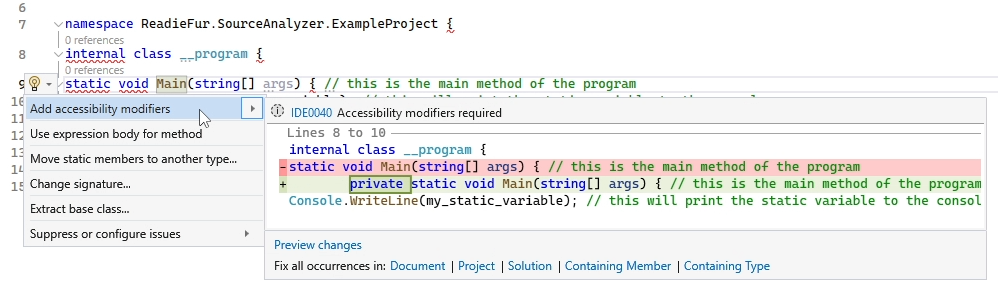
\includegraphics[width=0.5\textwidth]{Figures/IDEHintsCropped.png}
\end{wrapfigure}

Using the VSIX build of the project, a plugin compatible with the Visual Studio IDE was created. This plugin allowed for the tool to be interacted with via IDE hints. In order to examine this a test project was loaded up into Visual Studio with the plugin loaded. After compiling the project the IDE would gather diagnostics from the build tool and display them in the error list and the code editor. We can see that amongst the diagnostics generated, the tool has provided hints within the IDE that the user can click on to preview and apply the fix. This is shown in Figure \ref{fig:IDEHints}.

% TODO: Show the integration testing in action.

\subsubsection{Standalone testing}

\begin{wrapfigure}{r}{0.5\textwidth}
    \centering
    \caption{Standalone Tool}
    \label{fig:StandaloneTool}
    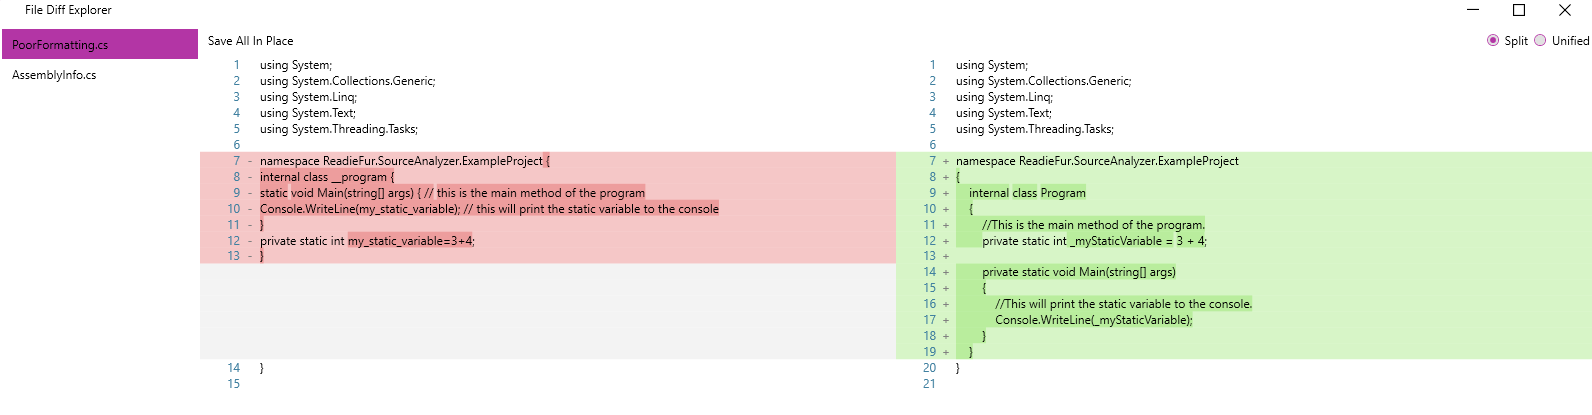
\includegraphics[width=0.5\textwidth]{Figures/StandaloneToolCropped.png}
\end{wrapfigure}

The standalone package was built to provide a way to run the tool without the need for the Visual Studio IDE. The standalone program is simplistic and takes a C\# solution file from which the analysis will be run on. Any files that can have fixes applied will be displayed in a graphical window with a file differential view. To validate the results of the standalone tool, checks were made to ensure that it doesn't get stuck in a read-eval loop which did occur during development. In addition to this the output files were visually inspected to check that the fixes were applied correctly (see Figure \ref{fig:StandaloneTool}).
